\chapter{Session-based programming and business protocols}
\label{chap:session-based-programming}

Communication is becoming a fundamental element of software development. Web applications increasingly combine numerous distributed services; an off-the-shelf CPU will soon host hundreds of cores per chip; corporate integration builds complex systems that communicate using standardized business protocols; and sensor networks will place a large number of processing units per square meter. A frequent pattern in communication-based programming involves processes interacting via some structured sequence of communications, which as a whole form a natural unit of conversation. In addition to basic message passing, a conversation may involve repeated exchanges or branch into one of multiple paths. Structured conversations of this nature are ubiquitous, arising naturally in server-client programming, parallel algorithms, business protocols, Web services, and application-level network protocols such as SMTP and FTP.

Objects and object-orientation are a powerful abstraction for sequential and shared variable concurrent programming. However, objects do not provide sufficient support for high-level abstraction of distributed communications, even with a variety of communication API supplements. Remote Method Invocation (RMI), for example, cannot directly capture arbitrary conversation structures; interaction is limited to a series of separate send-receive exchanges. More flexible interaction structures can, on the other hand, be expressed through lower-level (TCP) socket programming, but communication safety is lost: raw byte data communicated through sockets is inherently untyped and conversation structure is not explicitly specified. Consequently, programming errors in communication cannot be statically detected with the same level of robustness as standard type checking protects object type integrity.

In the previous chapter, thesis has explored a type theory for structured conversations in the context of process calculi and $\pi$-calculus. A session is defined as a conversation instance conducted over, logically speaking, a private channel, isolating it from interference; a session type is a specification of the structure and message types of a conversation as a complete unit. Unlike method call, which implicitly builds a synchronous, sequential thread of control, communication in distributed applications is often interleaved with other operations and concurrent conversations. Sessions provide a high-level programming abstraction for such communications-based applications, grouping multiple interactions into a logical unit of conversation, and guaranteeing their communication safety through types.

Further in the chapter, we will discover the impact of integrating session types into object-oriented environment like Java. Based on the work \cite{sessionbdpinjava}, \cite{sj-framework}, we will summarize the central features of the Session-Java (SJ) compilation-runtime framework:
\begin{compactenum}
\item  Integration of object-oriented and session programming disciplines. The thesis provides a good introduction of concise syntax for session types and structured communication operations in SJ. Session-based distributed programming involves specifying the intended interaction protocols using session types and implementing these protocols using the session operations. The session implementations are then verified against the protocol specifications. This methodology uses session types to describe interfaces for conversation in the way Java interfaces describe interfaces for method-call interaction.
\item Ensuring communication safety for distributed applications. Communication safety is guaranteed through a combination of static and dynamic validations. Static validation ensures that each session implementation conforms to a locally declared protocol specification; runtime validation at session initiation checks the communicating parties implement compatible protocols.
\end{compactenum}

\textit{Chapter summary.} Section \ref{sec:sj-intro} provides a fundamentals of SJ syntax and features. In section \ref{sec:scenarios} presents different scenarios to demonstrate power and efficiency of the language.

\section{Introduction to SJ}
\label{sec:sj-intro}

\underbar{The purpose:} To provide direct language support for (binary) session programming as an extension to Java.

Session programming starts from the description of protocols for interaction (using session types), which can then be concretely implemented using a set of structured communication operations available on session sockets. The SJ programs guarantees communication safety by:

\begin{compactenum}
\item  statically verifying that session implementations conform to the protocol specifications;

\item  a runtime compatibility validation between peers at session initiation.
\end{compactenum}

Session programming in SJ has the following benefits in comparison to widely used alternatives such as regular socket programming or Java RMI:

\begin{compactenum}
\item  Byte stream communication through raw network (TCP) sockets and the intended communication protocols have no direct representation in the program, neither as types nor programming constructs. These limitations can make programs more difficult to read and understand, and also to verify.

\item  RMI and other RPC-based technologies provide with fixed call-return shape of procedure call, that is not suited to expressing certain interaction patterns.
\end{compactenum}

Session programming is for systems and applications where the parties or components interact according to certain protocols: session types are formal specifications of such protocols. Session types describe structured sequences of interaction including basic message passing, branching, branching and repetition. A session is an instance of a session type, i.e. the unit of interaction encapsulating one run of a protocol. From the perspective of abstraction, each session, is conducted on a separate channel.

Session programming in SJ comprises the following stages:
\begin{compactenum}
\item design the protocols by which the parties should interact, and specify them as session types;

\item  the protocols are explicitly incorporated into the programs for each party or component: we declare the session types for the interactions to be performed;

\item  the actual interaction that comprise a session are implemented using the session programming constructs and operations. The session operations are performed like method calls on session socket objects, endpoint handles in the session channels (sockets).

\item  each session implementation is statically verified by the compiler according to the associated protocol specification (type system for session programming);

\item  session implementations must respect the property of session linearity (no session operations out of its scope) in terms of control flow and object aliasing.
\end{compactenum}

\subsection{Protocol Declaration}

Session programming begins by declaring the protocol for the intended interaction as follows:

\begin{equation*}
\text{protocol name \{\dots\}}
\end{equation*}
where name identifies the protocol, following the standard Java naming rules. Protocols may be declared as both local and field variables, although field protocols are currently restricted to private access. The body of the protocol is session type, given by the syntax rules in Table \ref{tab:sj-spec}, below.


\begin{longtable}{|p{0.15\textwidth}|p{0.3\textwidth}|p{0.3\textwidth}|}
\caption{SJ protocol specification}\label{tab:sj-spec} \\
\hline
$T$ & $::=T.T$ & Sequencing \\ \hline
& begin & Session initiation \\ \hline
& $!<M>$ & Message send \\ \hline 
& $?(M)$ & Message receive \\ \hline
& $\bigoplus \{L_1:T_1,\dots, L_n:T_n \}$ & Session branching \\ \hline
& $\bigoplus [T]*$ & Session iteration. \\ \hline 
& $\text{rec }L[T]$ & Session recursion scope. \\ \hline
& \#$L$ & Recursive jump. \\ \hline
& @$p$ & Protocol reference. \\ \hline
\end{longtable}

\begin{equation*}
\begin{array}{c}
M ::= \text{Object type } | \text{ Primitive type } | T \\
L ::= \text{Label} \\
\bigoplus ::= ! | ?
\end{array}
\end{equation*}

The session type specifies how a ~session should proceed in terms of the actions that the particular party should perform, i.e. a view of the session from the perspective of that party. The key point is that the implementation of a session is governed by the associated protocol: the SJ compiler statically verifies session implementations against the protocols. The kind of actions that can be specified include basic message passing, conditional and repeated behaviours. The session type elements that describe these actions are explained below in pairs according to the duality relation between corresponding elements. Session type duality ensures that two parties implement compatible protocols, checked through a runtime validation at session initiation. Duality essentially means when one session party is sending a message, the peer is (or will be) expecting a message of that type (or super type), thus precluding dynamic type errors from message communication.

\subsection{Interaction sequences and session initiation}

If $T$ and $T'$ are session types, then

\begin{equation*}
T.T'
\end{equation*}
is the session type that describes first performing the interactions of $T$ followed by the interaction $T'$.

The action of initiating a new session with a peer is denoted by:

\begin{equation*}
\text{begin}
\end{equation*}

Unlike most of the other session type constructors, `begin' is symmetric, meaning that both parties have the same specification of this action. Note that begin can only appear as the initial prefix at the top level of a session type, since a session can only be initiated once. It also worth noting, there is no explicit session type for the action of closing a session: the end of a session is implicit at the end of a type.

\subsection{Basic message passing, branching, iteration and recursion}

\begin{equation*}
!<M> \hspace{2cm} ?(M)
\end{equation*}

Sending and receiving a message of a type $M$ are respectively described by the dual types. Message types are serializable Java object types, primitive types and session types. The notion of duality between send and receive includes session sub-typing, which allows a message subtype to be sent where a super type is expected. In general, the `!' (`?') symbol in session types denotes some form of output (input) action, of which send (receive) is a particular instance.

Session can branch into one of multiple parts: one of the parties is responsible for making the branch decision (which path to select) and the other party must follow. Paths are identified by string labels:

\begin{equation*}
!\{L_1:T_1,\dots, L_n:T_n\} \hspace{2cm} ?\{L_1:!T_1,\dots, L_n:!T_n \}
\end{equation*}

The type on the left specifies that the session party is decision maker and may select one of the paths labeled from $L_1$ to $L_n$. The dual type on the right (where $!T_x$ is dual type of $T_x$), says the session peer should follow the first party's decision and take the corresponding path. The type below means that whichever branch is selected, the session, will then proceed according to the type $T'$ after the branch has been completed.

\begin{equation*}
\begin{array}{c}
\bigoplus \{L_1:T_1,\dots, L_n:T_n\}.T' \\
![T]* \hspace{2cm} ?[!T]*
\end{array}
\end{equation*}

Sessions may involve the iteration of some subsession. Similarly to branching, one session party is responsible for making the decision at each iteration whether or not to iterate, and the session peer must follow. The decision to iterate or not is made before each iteration, so the sub-session may be performed zero or more times.

Repeated behaviour in session types can also be specified using recursion

\begin{equation*}
\text{rec }L[T] \hspace{2cm} \# L\text{ may occur in }T
\end{equation*}
where $L$ is alphanumeric label and `\#' is just a symbol which essentially means ``jump'' back to the protocol state at which the label was declared (rec $L$) and repeat \textit{T}. Recursions with different labels can be nested: can jump back out to any nesting level specifying the appropriate label.

\subsection{Higher order message types}

As mentioned above, message types can themselves be session types. The higher-order communication types additionally express changes in the shape of the session network. For example, the dual types

\begin{equation*}
!<?(\text{int})> \hspace{2cm} ?(?(\text{int}))
\end{equation*}

\begin{figure}
\centering
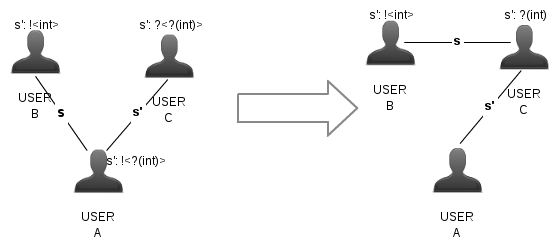
\includegraphics[width=0.8\textwidth]{resources/sj_delegation_session.png}
\caption{Session delegation}\label{fig:sj-delegation}
\end{figure}

respectively says that we should send and receive a session of type ?(int). Higher order session communication is often referred to as session delegation. figure \ref{fig:sj-delegation} shows a basic delegation scenario. The left part illustrates the session configuration before the delegation is performed: UserB engaged in a session $s$ of type $!<$int$>$ with UserA, while UserA is also involved in a session $s'$ with UserC of type $!<?($int$)>$. So, instead of accepting the integer from UserB himself, UserA delegates his role in $s$ to UserC, so that he will receive this message. This delegation action corresponds to UserA's higher-order send type for the session $s'$ with UserC. The right part of figure illustrates the change in session configuration after the delegation has been performed: UserB now directly interacting with UserC for the session $s$.

An important property of delegation is that the type of session being delegated does not itself convey any information about the delegation: the delegation action is between UserA and UserC, and is transparent to UserB, the passive party. Because UserC will fulfill the session contract originally signed by UserA, session delegation keeps communication safety.

Another useful application of higher-order session types is the communication of types like

\begin{equation*}
!<\text{begin}.T> \hspace{2cm} ?<\text{begin}.T>
\end{equation*}
Since the nested session type is prefixed by begin, the session has not yet been initiated. This communication informs the recipient about another peer from which new sessions of the specified type may be requested. This permits the creation of new edges in a session configuration as well as migration of existing edges. This type of action arises naturally in many real world settings, such as FTP.

For syntactic convenience, one protocol can be referenced from another using the @ operator. For example, given protocol $p1\{\dots\}$, we can write protocols like protocol  $p2{\dots .@p1 \dots}$ or protocol $p3{\dots !<@p1> \dots}$ or $p{\rm 2\ }{\rm \{}{\rm \dots .@}p{\rm 1\ \dots }{\rm \}}$, where The $@p$ is syntactically substituted for the protocol of that name. Protocols cannot make reference themselves, nor forward references.

\subsection{Session sockets}

Session sockets are implementing the actual session code according to the specified session type (protocol). They are represent the endpoints (participants) of a session connection: each of the parties owns one endpoint and performs the specified interactions via the SJ session operations on that endpoint.

In SJ session sockets are objects that extend the abstract \textit{SJSocket} class. \textit{SJRSocket::SJSocket} and \textit{SJFSocket::SJSocket}, both, employ TCP as underlying transport. SJ is distinguishing session client and server sockets, where the former are used to request sessions from the latter.

Session client sockets are created by calling the static \textit{create} method on the used socket class, \textit{SJFSocket} or \textit{SJRSocket}. This method takes as a parameter an object of type \textit{SJServerAddress}, which binds the IP address and TCP port of the target session server with the type of the session supported by that server. SJServerAddress objects are also created by calling a static create method on the class, passing as parameters the information just described. For example, assuming the protocol $p$ already defined,

\begin{lstlisting}
SJServerAddress c = SJServerAddress.create(p, "host", 1234);
SJSocket s        = SJFSocket.create(c); // Or use SJRSocket.
\end{lstlisting}
first creates the session server address $c$, associated with the protocol (session type) $p$. $c$ is then used to create a session socket $s$, which means that $s$ should be used for sessions of type $p$ with specified server by port number and hostname. An important requirement in SJ is that session-typed objects, such as SJSocket and SJServerAddress, are not permitted to be aliased. In particular, assignment both from and to session-typed variables is forbidden, as is passing the same session-typed variable as multiple arguments in the same method call. Session client sockets cannot be ``reused'', i.e. once a session has been completed, it cannot be run again using the same session socket object.

Session server-sockets are the counterpart to the above session (client) sockets. Session server-sockets are created in much the same way,

\begin{lstlisting}
SJServerSocket ss = SJFServerSocket.create(q, 1234); // 'q' is a protocol.
\end{lstlisting}
but are created active, meaning that the specified port is opened and \textit{ss} is immediately read to accept session requests.

Sessions are implemented within session-try statements. Session-try is very similar to the regular Java try, but also takes as parameters the session sockets for sessions that may be implemented within its scope. Also, any sessions initiated within a session-try must be completed within the session-try scope.

\begin{lstlisting}
try (s1, s2) { 
... // someop
} catch () {
... // catching exc
} finally {
... // session closing
}
\end{lstlisting}

As for regular try statements, the finally clause is optional if there is a catch clause, and vice versa. The implementations of $s1$ and $s2$ may be interleaved along with other Java code, provided that they respect their protocols and the other rules of the session type system. The SJ compiler statically checks that initiated sessions are completed within parent session-try according to the relevant protocols. The completion of the session can be designated by:

\begin{compactenum}
\item  session delegation;

\item  session passing as an argument to another SJ session;

\item  spawning in SJ session thread.
\end{compactenum}

\subsection{Session operations}

After creating a protocol (session type) and a session socket that intended to implement that protocol, the session can be implemented within a session-try using the \textit{session operations}, depicted in Table \ref{tab:session-ops}.

\begin{longtable}{|p{0.4\textwidth}|p{0.4\textwidth}|}
\caption{Session operations specification}\label{tab:session-ops}\\ \hline
s.request() & begin \\ \hline 
s.send(m) & $!<M>$ \\ \hline
s.receive() & $?(M)$ \\ \hline
s.outbranch(L) \{P\} & $!\{L:T\}$ \\ \hline
s.inbranch() \{case L1: {P1}\dots case Ln:{Pn}\} & $?\{L_1:T_1,\dots, L_n:T_n\}$ \\ \hline
s.outwhile(cond) \{P\} & $[T]*$ \\ \hline
s.inwhile() \{P\} & $?[T]*$ \\ \hline
s.recursion(L) \{P\} & rec $L[T]$ \\ \hline
s.recurse(L) & $\#L$ \\ \hline
\end{longtable}

The session operations are invoked via session sockets in a method call-like manner. To delegate a session, the session socket variable must be passed to a send operation on the target session.

\begin{lstlisting}
s1.send(s2) // !<T>, where T is the remaining session type of 's2'
\end{lstlisting}

Only active session sockets can be delegated, and delegation implicitly completes the delegated session. The receive operation receives delegated sessions:

\begin{lstlisting}
SJSocket s2 = s1.receive()
\end{lstlisting}

Casts are optional, as for ordinary receive operations.

\begin{lstlisting}
s2 = (T1) s1.receive()
s3 = (@p) s1.receive() // ?(T2), where T2 is the session type declared by p
\end{lstlisting}

Session sockets can be passed as arguments to, and returned from, session methods. Session methods are the same as regular methods, except the parameter or return type for session values should the expected session type. The following is an example session method that takes a session type and additional parameters:

\begin{lstlisting}
try(s1) {
    ... // impl of s1
    finishSession(s1, 1, "hello world");
}
private void finishSession(T1 session, int cnt, String msg) throws SJIOException {
    ... // finish session according to protocol 'T1' 
}
\end{lstlisting}

The key point is that the type of session argument \textit{session}, $T1$, must correspond to the remainder of the session $s1$ at the point of the method call. Session-try scope is served implicitly in session calling method. By the standard rules for exceptions, any exceptions that may be raised by the session operations used, such as SJIOException must be thrown out by the method back to the parent session-try. The next example returns a session from a session method. The session $s2$ is initiated and partially implemented within \textit{getSession} before it is returned to the calling context, where the remainder of the session is implemented.

\begin{lstlisting}
try (sret) {
    ... // 'sret' is null-initialised and not yet assigned to. sret = getSession(123);
    ... // finish 'sret' according to 'T2'.
}
...
private T2 getSession(int i) throws ... { // Multiple exceptions.
    ... // 's2' created. 
    try (s2) {
        ... // 's2' partially implemented.
        return s2; // 's2' has remaining type 'T2'. 
    }
    finally { ...
    }
}
\end{lstlisting}


\section{Business case studies}
\label{sec:scenarios}

V3na.com is an e-commerce web portal that sells SaaS applications for business needs. V3na has developed on Django framework (Python)\footnote{ Django is a high-level python web framework that encourages rapid development and clean. Further information: \url{https://www.djangoproject.com/}}. The persistence layer is based on MongoDB and Memcached. One of the challenging task was to automate the process of SaaS integration. By integration we understand the following processes with a particular SaaS application:

\begin{compactenum}
\item  connection: SaaS user can connect SaaS for trial period by simply clicking on the button;

\item  subscription extension and freezing;

\item  payment confirmation;
\end{compactenum}

Before all the formalisms will be discovered, it is a good starting point to specify simple business protocol of one of the processes just mentioned. For instance, informally the expected process of SaaS connection may be interpreted as follows:

\begin{compactenum}
\item  SaaS User asks V3na, through a specified channel, to connect particular SaaS application for trial period.

\item  V3na service checks that user has an active session with V3na. If so, V3na replies with the messages ``SaaS connecting. Wait for couple of minutes''. At the same time, V3na builds ``User connection'' request to this SaaS.

\item  SaaS handles the request from V3na: validates message structure, verifies message integrity. After the steps of validations-verifications, SaaS either creates an account with new user for trial period and responds V3na with status ``OK'' or refuses the request because of failure and responds V3na with status ``FAIL''.

\item  Depending on SaaS response, V3na sends ``OK'' or ``FAIL'' message to originally requesting User.
\end{compactenum}

\begin{figure}
\centering
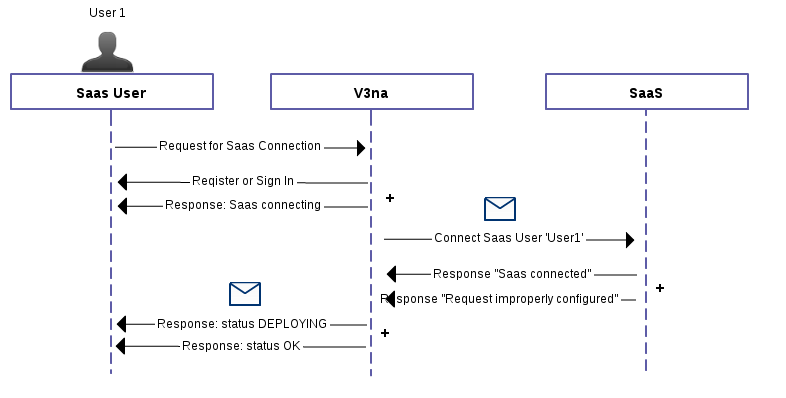
\includegraphics[width=0.8\textwidth]{resources/v3na-protocol.png}
\caption{V3na protocol for SaaS connection}
\label{fig:v3na-protocol}
\end{figure}


figure \ref{fig:v3na-protocol} presents an UML sequence diagram of the connection protocol. Many details are left unspecified: in real interaction, there specified the type of messages exchanged, security protocol, message structure and so on. Further, the communication can be represented through the sessions. In order to represent the communication through the sessions, the following assumptions have to be considered according to \cite{structured-com-centered-prog}:

\begin{compactenum}
\item  SaaS User, V3na and SaaS are called \textit{participants};

\item  Each participant communicates through the channels

\item  Dual communication --- a sender sends a message and receiver receives it

\item  Communication can be in-session communication, which belongs to a session, or session initiation channels which establishes a session
\end{compactenum}

In the next subsections, I will present the three case studies, increasing in complexity and reflecting the central aspects of session-based programming.

\subsection{Scenario \# 1}

This scenario corresponds to the description of connecting user to SaaS on v3na.com in previous section. The scenario is as follows:

\begin{enumerate}
\item  User begins a request session (s) with cloud service (V3na) and sends the request ``Connect SaaS'' as JSON-encoded message.

\item  V3na sends either:

\item  FAIL, if user has no active session (not signed in on V3na) and further interaction terminates 

\item  OK, if user has logged in and request data has passed validation steps. Then Cloud initiates a new session (s') with SaaS and requests it for new user connection with HttpRequestJSONMessage.

\item  If OK label take place, Cloud initiates a new session (s') with SaaS and requests it for new user connection with HttpRequestJSONMessage. finally SaaS responds to Cloud with connection status (OK, FAIL) and V3na sends this status to User. Both sessions have to be terminated.
\end{enumerate}

\textbf{Protocols.} The decision in the protocol will be incorporated through the use of outbranch. So the whole scenario is presented on Table \ref{tab:protocols-sc1}.

{\lstset{
framerule=0pt,
numbers=none
}
\begin{longtable}{|p{0.25\textwidth}|p{0.25\textwidth}|p{0.25\textwidth}|}
\caption{Protocols of scenario \# 1}
\label{tab:protocols-sc1} \\ \hline
\textbf{User} & \textbf{Cloud (V3na)} & \textbf{SaaS} \\ \hline
\endhead

\begin{lstlisting}
protocol p_uv { 
  begin.
  !<JSONMessage>. 
  ?{
    OK: ?(JSONMessage).?(int),
    FAIL: 
  }
}
\end{lstlisting}
&
\begin{lstlisting}
p_vu { 
  begin.?(JSONMessage).!{
    OK: !<JSONMessage>.!<int>,
    FAIL: 
  }
protocol http_req_rep {
  !<JSONMessage>.
  ? (JSONMessage)
}
protocol p_vs { 
  begin.@http_req_rep 
}
\end{lstlisting}
&
\begin{lstlisting}
protocol p_sv { 
  begin.
  ?(JSONMessage). !<JSONMessage> 
}
\end{lstlisting}
\\ \hline
\end{longtable}
}

\textbf{Interactions. } The general syntax for global description has been interpreted into a sequence UML diagram, as depicted in figure \ref{fig:interaction-overview-sc1}. The whole syntax is on the down-left side of the figure. In case of choice, terminated branches are out of scope of the main picture, but still a subpart of the whole diagram. Next step is implementation of this diagram in Session-Java.

\begin{figure}
\centering
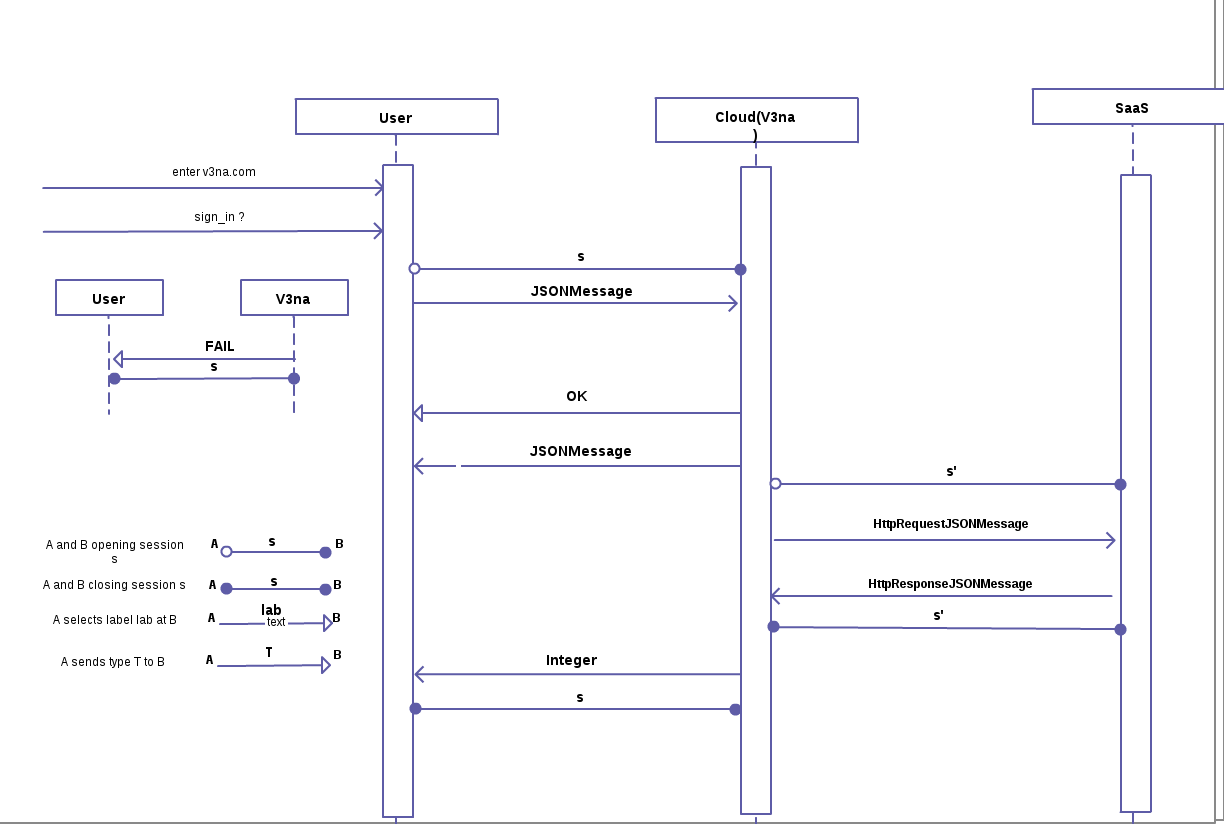
\includegraphics[width=0.8\textwidth]{resources/interaction-sc1.png}
\caption{Overview of interactions for Scenario \# 1}
\label{fig:interaction-overview-sc1}
\end{figure}

The main concept of SJ is that User choice reflected through the outbranch case. For the full source code, refer to Appendix \ref{app:sc1} or repository \cite{thesis}.

\subsection{Scenario \# 2}

New scenario is a bit harder in complexity, and a loop and session delegation features are introduced. The description of this scenario presented below:

\begin{compactenum}
\item  User begins a request session (s) with cloud service (V3na)

\item  V3na asks User to login, so next User provides V3na with login and password Strings.

\item  V3na receives User credentials and verifies them: If User is authenticated with minimal amount of tries or amount of tries is out of limit, he is allowed to continue further interactions with V3na, otherwise --- not. Go back to step 2.

\item  If User is not allowed to access V3na, the interaction between User and V3na continues on DENY-branch, otherwise --- on ACCESS-branch.

\item  If next branch is ACCESS, User sends his connection request with details to V3na. V3na creates new session with SaaS (s') and delegates the remaining session s with User on the latter and sends last user request details. Session s' is terminated.

\item  SaaS continues interaction with user by session s. By steps of validation-verification, SaaS either responds User to proceed interaction by branch OK or FAIL. In both cases User receives from SaaS directly the reason and status of his request. Session s is terminated.
\end{compactenum}

\textbf{Protocols.} first of all, the protocol provided with iterations using $![\dots]*$ $?[\dots]*$. Then protocol introduces higher order operations of type $!<T>\ \ ?<T>$. Full description is provided in tables \ref{tab:user-cloud-protocols} and \ref{tab:cloud-saas-providers}.

{
\lstset{
framerule=0pt,
numbers=none
}
\begin{longtable}{|p{0.4\textwidth}|p{0.4\textwidth}|}
\caption{User-Cloud protocols}\label{tab:user-cloud-protocol} \\ \hline
\textbf{User} & \textbf{Cloud} \\ \hline \endhead
\begin{lstlisting}
protocol p_uv { 
  begin.?[!<String>.!<String> ]*.
  ?{
   ACCESS: !<JSONMessage>.
   ?{
     OK: ?(JSONMessage), FAIL: ?(JSONMessage)
   },
  DENY: ?(String)
  } 
}
\end{lstlisting}
&
\begin{lstlisting}
private protocol p_vu { 
  begin.
   ![ ?(String).?(String) // login password
     ]*.
  !{
    ACCESS: ?(JSONMessage).
    !{
      OK: !<JSONMessage>, FAIL: !<JSONMessage>
     },
      DENY: !<String>
   } 
}
\end{lstlisting}
\\ \hline
\end{longtable}
}


{
\lstset{
framerule=0pt,
numbers=none
}
\begin{longtable}{|p{0.4\textwidth}|p{0.4\textwidth}|}
\caption{Cloud-SaaS protocols}\label{tab:cloud-saas-providers} \\ \hline
\textbf{Cloud} & \textbf{Saas} \\ \hline \endhead
\begin{lstlisting}
protocol p_vs {
  begin.
  !< !{
    OK: !<JSONMessage>, 
    FAIL: !<JSONMessage>
  } >.!<JSONMessage>    
}
\end{lstlisting}
&
\begin{lstlisting}
protocol p_msg { 
  !{
    OK: !<JSONMessage>,
    FAIL: !<JSONMessage> 
  }
}

protocol p_sv {
  begin.?(@p_msg).?(JSONMessage) 
}
\end{lstlisting}
\\ \hline
\end{longtable}
}

Unlike the previous protocol, the Cloud-Saas protocol significantly altered, also authentication process is added to the protocol in interaction between User --- Cloud. It is important to note that 

\begin{lstlisting}
!<
    !{
        OK: !<JSONMessage>,
        FAIL: !<JSONMessage> 
    }
>
\end{lstlisting}
corresponds to a higher-order message. The !$<\dots>$ means that it is the Cloud that is passing the high order message and everything inside it is the protocol of the session that Saas should perform with the User. In Saas --- Cloud, the protocol defined in more subtle way containing higher order messages by first defining them and then including them in the protocol. For syntactic convenience, one protocol can be referenced from another using @ operator. The $@p$ is syntactically substituted for the protocol of that name.

\begin{figure}
\centering
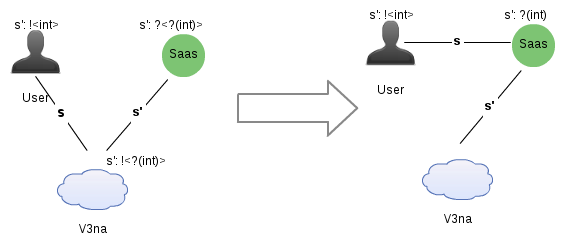
\includegraphics[width=0.8\textwidth]{resources/sj-delegation.png}
\caption{Session delegation in Scenario \# 2}
\label{fig:session-delegation-sc2}
\end{figure}

\textbf{Interactions.} figure \ref{fig:session-delegation-sc2} shows the general picture of session delegation for scenario 2. The left picture is before the session delegation, while the right picture is the state after delegation. figure \ref{fig:seq-diagram-sc2} depicts the protocols provided above using an UML sequence diagram. The language of the artifacts has already presented in the first scenario.

\begin{figure}
\centering
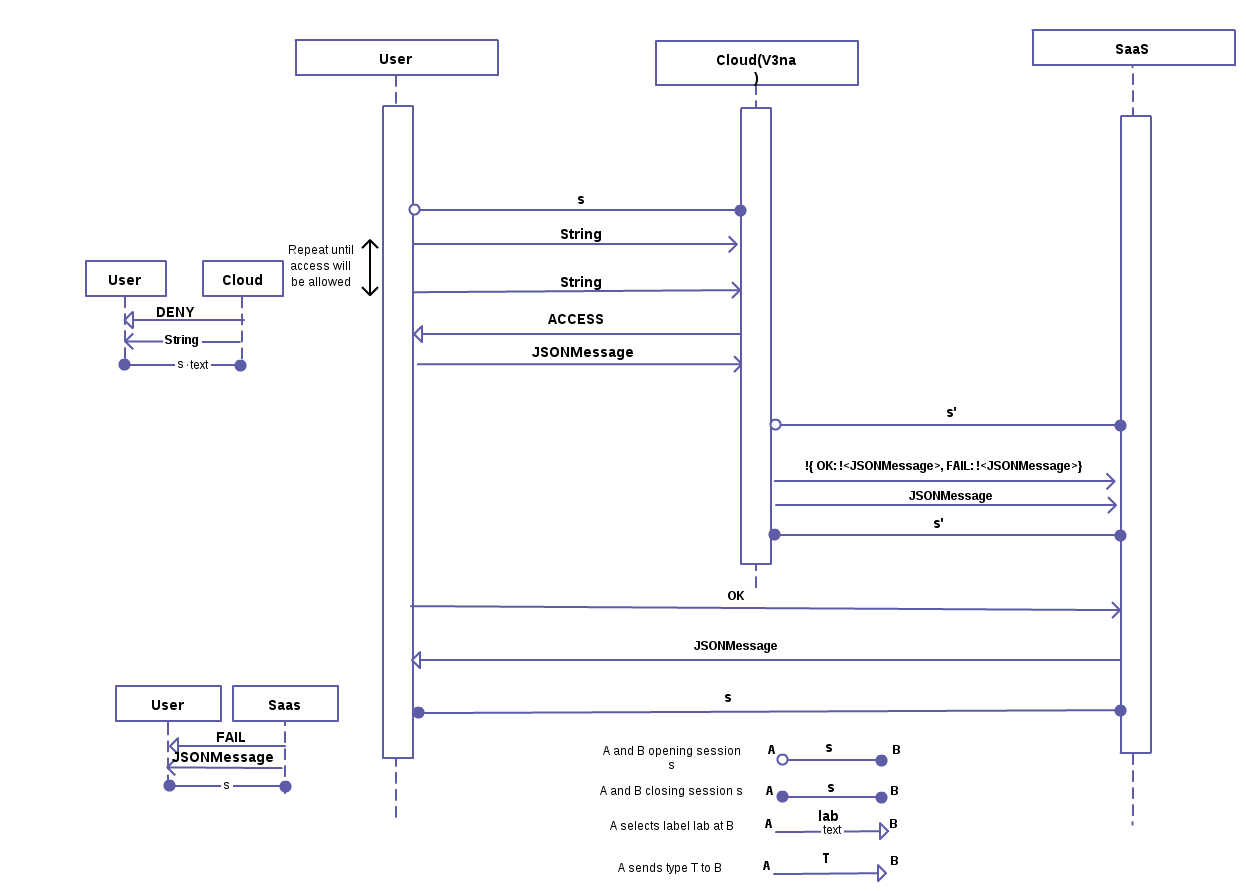
\includegraphics[width=0.8\textwidth]{resources/interaction-sc2.png}
\caption{Sequence diagram of interactions for Scenario \# 2}
\label{fig:seq-diagram-sc2}
\end{figure}

\textbf{Implementation}. Despite the fact that session delegation takes place, the program still remains very simple. Actually delegating the protocol is straightforward and only consists of passing the socket to service:

\begin{lstlisting}
s_vs.send(user_vu); // pass the remaining protocol
\end{lstlisting}

I have decided to include the whole segment of code to illustrate the following point. 

\begin{lstlisting}
user_vu.outbranch(ACCESS) {
  JSONMessage req_info = user_vu.receive(); SJServerAddress addr_vs = SJServerAddress.create(p_vs, saas_hname, saas_port);
  SJSocket s_vs = SJRSocket.create(addr_vs); try(s_vs) {
    s_vs.request();
    s_vs.send(user_vu); // pass the remaining protocol    
    s_vs.send(req_info);
  } catch(UnknownHostException uhe) {
    uhe.printStackTrace(); 
  }
}
\end{lstlisting}

To receive a high order message type casting must take place in the case of a protocol, the type of protocol must be explicitly defined:

\begin{lstlisting}
v3na_user_socket = (@p_msg) v3na_sv.receive();
\end{lstlisting}

Where p\_msg is defined in the protocols section. This is a reason why it is good practice to first exclusively write the protocol to be delegated and then include it in the final protocol. For the full source code, refer to Appendix \ref{app:sc2} or repository \cite{thesis}.

\subsection{Scenario \# 3}

This is a new scenario, devoted to payment and wallet recharging processes analysis developed for V3na.com \cite{v3na}. The description of this scenario is defined below as follows:

\begin{enumerate}
\item  User begins a request session (s) with cloud service (V3na)

\item  V3na asks User to login, so next User provides V3na with login and password strings.

\item  V3na receives User credentials and verifies them: If User is authenticated with minimal amount of tries or amount of tries is already out of limit. In first case, he will be allowed to continue further interactions with V3na, in second case -- he will not. Go back to previous step.

\item  If User is not allowed to access V3na, the interaction between User and V3na continues on DENY-branch. User receives the error message and protocol is terminated.

\item  If next branch is ACCESS, User proceeds with payment or wallet recharging interactions.

\item  If user chooses PAYMENT: 

\begin{enumerate}
\item  Cloud delegates the remaining interaction of session s to the payment backend via session s'.

\item  As response from the payment backend, User receives the Goods collection that have to  be payed. User chooses either Visa/Mastercard or Non-cash payment way. In both cases User sends his private details: card or transfer details. 

\item  finally User receives the status of his payment and session s terminated
\end{enumerate}

\item  If user chooses WALLET:

\begin{enumerate}
\item  Cloud delegates the remaining interaction of session s to the wallet backend via session s'.

\item  Wallet backend continues interaction with User. User sends taxation number and then his wallet id. 

\item  Wallet backend verifies by taxation number that payment is active and checks by wallet id that user exists.

\item  finally Wallet backend notifies user with status of wallet recharging and session s is terminated.
\end{enumerate}
\end{enumerate}

\textbf{Protocols.} Calculating the protocols for this scenario is a little different than what has been shown before. In the current scenario the session between Cloud and Cloud backends (Payment, Wallet) involves the Cloud delegating the session with the User to one of those backends. It is similar to an application server behavior, while dealing with multiple clients it must delegate particular work on the its components. The protocol definition includes four protocols (participant per protocol). The protocols are provided in tables \ref{tab:user-cloud-protocols} and \ref{tab:cloud-payment}.

{
\lstset{
framerule=0pt,
numbers=none
}
\begin{longtable}{|p{0.4\textwidth}|p{0.4\textwidth}|}
\caption{User, Cloud protocols}\label{tab:user-cloud-protocols} \\ \hline
\textbf{User} & \textbf{Cloud} \\ \hline \endhead
\begin{lstlisting}
protocol payment { ?(Goods).!{
  VISA_MASTER: !<CardDetails>,
  TRANSFER: !<TransferDetails> }.?{
    PAID: ?(String), DECLINED: ?(String), FAILED: ?(String)
  } 
}
private static protocol wallet { 
  ?(String).!<Integer>.!<Integer>.?{
    PAYMENT_INACTIVE: ?(OSMPMessage),
    USER_NOT_FOUND: ?(OSMPMessage),
    OK: ?(OSMPMessage) 
  } 
}
private static protocol p_uv {
  begin.?[ !<String>.!<String>
  ]*.?{
    ACCESS: !{
      PAYMENT: @payment,
      WALLET: @wallet 
    },
    DENY: ?(String) 
  }
}
\end{lstlisting}
&
\begin{lstlisting}
protocol p_payment { 
  !<Goods>.?{
    VISA_MASTER: ?(CardDetails),
    TRANSFER: ?(TransferDetails) 
  }.!{
    PAID: !<String>, DECLINED: !<String>, FAILED: !<String>
  } 
}
protocol p_wallet { 
  !<String>.?(Integer).?(Integer).!{
    PAYMENT_INACTIVE: !<OSMPMessage>, USER_NOT_FOUND:
    !<OSMPMessage>, OK: !<OSMPMessage>
  }
}
protocol p_vp {
  begin.!<String>.!< @p_payment > 
}
protocol p_vw {
  begin.!<String>.!< @p_wallet >
}
\end{lstlisting}
\\ \hline
\end{longtable}
}

{
\lstset{
framerule=0pt,
numbers=none
}
\begin{longtable}{|p{0.4\textwidth}|p{0.4\textwidth}|}
\caption{Cloud backends protocols: Payment, Wallet}\label{tab:cloud-payment} \\ \hline
\textbf{Payment Backend} & \textbf{Wallet Backend} \\ \hline \endhead
\begin{lstlisting}
private protocol p_payment { 
  !<Goods>.?{
    VISA_MASTER: ?(CardDetails),
    TRANSFER: ?(TransferDetails) 
  }.!{
    PAID: !<String>, DECLINED: !<String>, FAILED: !<String>
  } 
}
private protocol p_pv { begin.?(String).?( @p_payment ) }
\end{lstlisting}
&
\begin{lstlisting}
private protocol p_wallet { 
  !<String>.?(Integer).?(Integer).!{
    PAYMENT_INACTIVE: !<OSMPMessage>,
    USER_NOT_FOUND: !<OSMPMessage>,
    OK: !<OSMPMessage> 
  }
}
private protocol p_wv { begin.?(String).?( @p_wallet ) }
\end{lstlisting}
\\ \hline
\end{longtable}
}

\textbf{Interactions.} After the delegation of session $s$ is performed, the interaction of User-PaymentBackend and User-WalletBackend is provided on separate pictures of figure \ref{fig:interaction-sc3}.

\begin{figure}
\centering
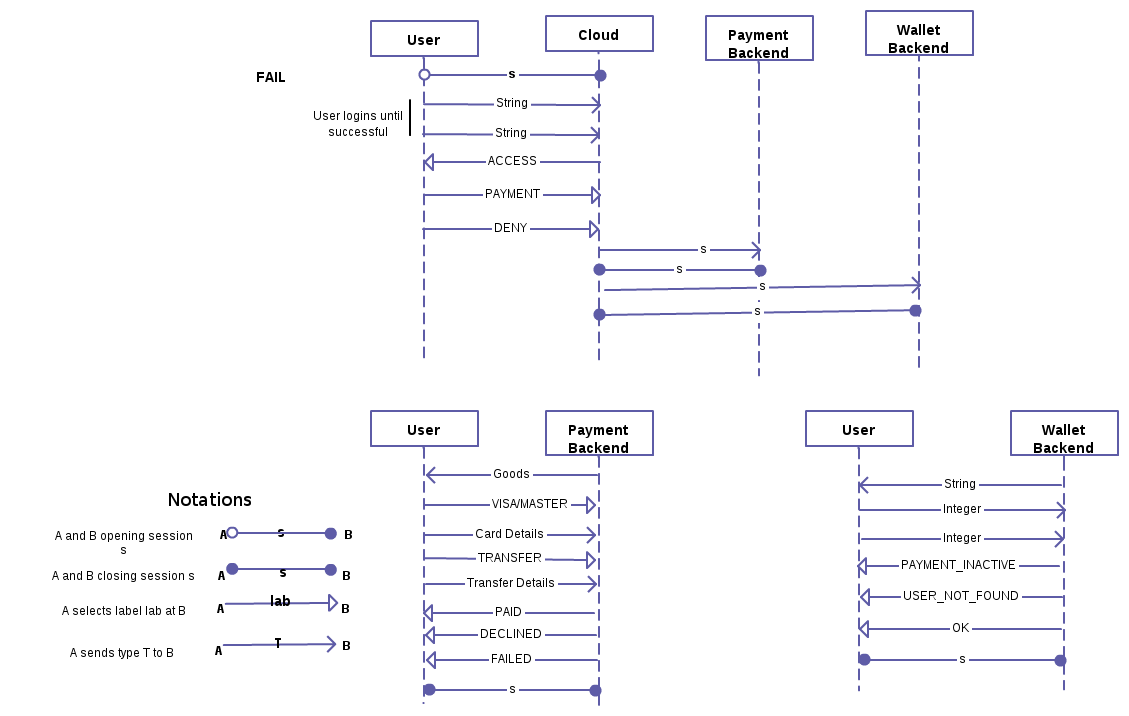
\includegraphics[width=0.8\textwidth]{resources/interaction-sc3.png}
\caption{Choreography for Scenario \# 3}
\label{fig:interaction-sc3}
\end{figure}

\textbf{Implementation. } Although the scenario is quite trivial, the tricky part is actually establishing the session between two parties. All interactions are passed into parallel thread using the \textit{spawn} operation. Session threads extend the \textit{sj.runtime.net.SJThread} class. Like \textit{java.lang.Thread}, SJThread must declare a single public void run method containing the thread body.

\begin{lstlisting}
s_pu>.spawn(new PaymentTransactionThread(username));
<s_wu>.spawn(new WalletRechargeTransactionThread(username));
\end{lstlisting}

For the full code, refer to \cite{thesis}.

These scenarios are an example of a business offering web services similar to the way many businesses operate. These scenarios has implemented using the concepts of Session-based programming in Object-Orientated programming through the original implementation by Raymond Hu.

In different scenarios, the Master thesis underlines the process of implementing a scenario in stages.

\begin{compactenum}
\item  Beginning from the design stage, the programmer must first consider how interactions between all parties participating in the scenario should be formed.

\item  Next the protocols have to be defined accordingly, with attention given to the duality of each session.

\item  By implementing the protocols the main skeleton of the program will have been completed

\item  Any local computations and other properties of the programs not regarding the sessions can then be coded.
\end{compactenum}

As the scenarios increase in size and complexity, directly implementing the protocols after we have defined them might be an awesome task. It would be quite helpful if at first the programmer deals with trivial protocols, to achieve compilation of the program with all the sessions set up, and only then moving on to implement the correct protocols. I tried to show that any set of interactions between two parties can be directly transformed into an SJ protocol. Mastering this is an important basis for a programmer wishing to move on with Session-based programming.

An effort was also given into using as many of the SJ session types as possible. Some examples are \textit{inbranch - outbranch}, \textit{outwhile - inwhile}, \textit{delegation}. I tried to use these constructs in a variety of ways in order to identify any problems with the compiler (but failed to find anything worth mentioning), although SJ is still in development. A couple of minor points would be that it is currently necessary that for any if statement we include an else, regardless of whether it is empty or not. Otherwise the compiler will bring an error message. 